\section{Profil utilisateur}
\label{sec:profil}

Le compte utilisateur est une fonctionnalité qui va permettre à l'utilisateur de faciliter sa navigation sur le site. En effet, les revues seront reliées à un créateur et des contributeurs. Ainsi, les utilisateurs retrouveront la liste des revues créées et contribuées lorsqu'ils voudront ajouter l'article qu'ils sont en train de visualiser à une revue. Cela rend l'ajout d'articles beaucoup plus simple car l'utilisateur ne sera pas obligé de rechercher, à chaque fois, les revues auxquelles il participe souvent. De plus, il pourra marquer les articles pour pouvoir les retrouver facilement plus tard.

\subsection{Apports}
\label{apport}
 

Un utilisateur qui disposera d'un compte aura accès à plusieurs fonctionnalités :

\begin{itemize}
  \item Avoir un compte utilisateur permet de créer des revues de presse ainsi que d'ajouter des articles aux revues.
	\item Si on est le créateur d'une revue, on peut changer l'ordre des articles et les retirer de la revue. Il sera aussi possible de supprimer la revue.
  \item Un ajout plus rapide d'un article à une revue qu'on a créée ou contribuée.
  \item Marquer des articles afin de pouvoir les retrouver facilement si l'utilisateur souhaite les relire plus tard. Ces articles seront rangés dans une liste appelée "Articles favoris". Il pourra par la suite les retirer de ses favoris.
	\item Ajouter ou supprimer des tags sur les articles.
\end{itemize}

En revanche, il n'est pas obligatoire d'avoir un compte utilisateur. Une personne qui n'a pas de compte peut tout de même rechercher un article ou une revue de presse dans la base de données. Elle pourra aussi visualiser les documents ainsi que consulter les revues de presse. Mais elle ne pourra pas créer une revue de presse ni y ajouter des articles.


\subsection{Création d'un compte}
\label{creation_compte}


La création d'un compte se fera de la même manière que font d'ores et déjà la majorité des sites web. L'utilisateur devra entrer un pseudonyme, une adresse mail et un mot de passe. Il recevra ensuite un mail afin de confirmer la création du compte. La présence de l'adresse mail permettra de surcroît d'avoir une fonctionnalité "mot de passe oublié ?" permettant à l'utilisateur de pouvoir mettre un nouveau mot de passe pour son compte s'il a oublié le mot de passe courant.


\subsection{Espace utilisateur}
\label{espace_util}

Lorsque l'utilisateur est connecté, il pourra accéder à un espace utilisateur. Dans cet espace, l'utilisateur pourra voir la liste des articles qu'il a marqués. Cette liste sera sous forme de menu déroulant. Une partie des articles sera affichée mais l'utilisateur pourra voir le reste de la liste en cliquant sur les flèches qui se trouvent de part et d'autre du menu. Pour chaque article, il sera indiqué le titre de celui-ci, le nom du journal et la date. Le début de l'article sera aussi affiché. En cliquant sur l'un des articles de la liste, l'utilisateur arrivera sur la page de visualisation de l'article. Il aura aussi accès à la liste des revues qu'il a créée et celles auxquelles il a contribué. Ces listes se présenteront de la même façon que pour la liste des articles marqués. Pour chaque revue, le nom de celle-ci sera indiqué. L'utilisateur pourra aller sur la page d'une des revues de presse en cliquant dessus. Il y aura aussi un lien pour pouvoir créer une nouvelle revue de presse. 
Enfin, un lien redirigeant vers la page permettant de modifier ses paramètres sera présent. Sur cette page, l'utilisateur pourra changer son mot de passe ainsi que son adresse mail.

    \begin{figure}[H]
        \centering
        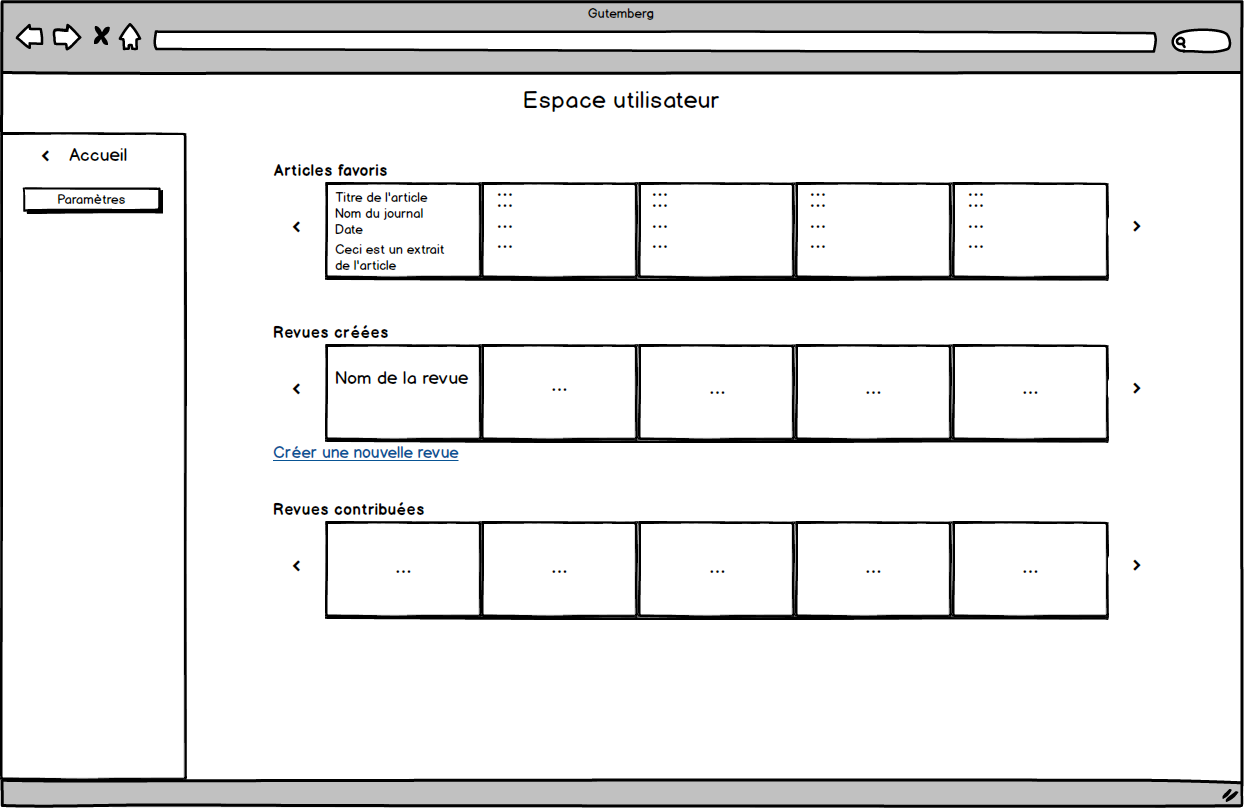
\includegraphics[width=\textwidth]{figures/Utilisateur.png}
            \caption{Page d'un profil utilisateur}
            \label{fig:utilisateur}
    \end{figure}

    \begin{figure}[H]
        \centering
        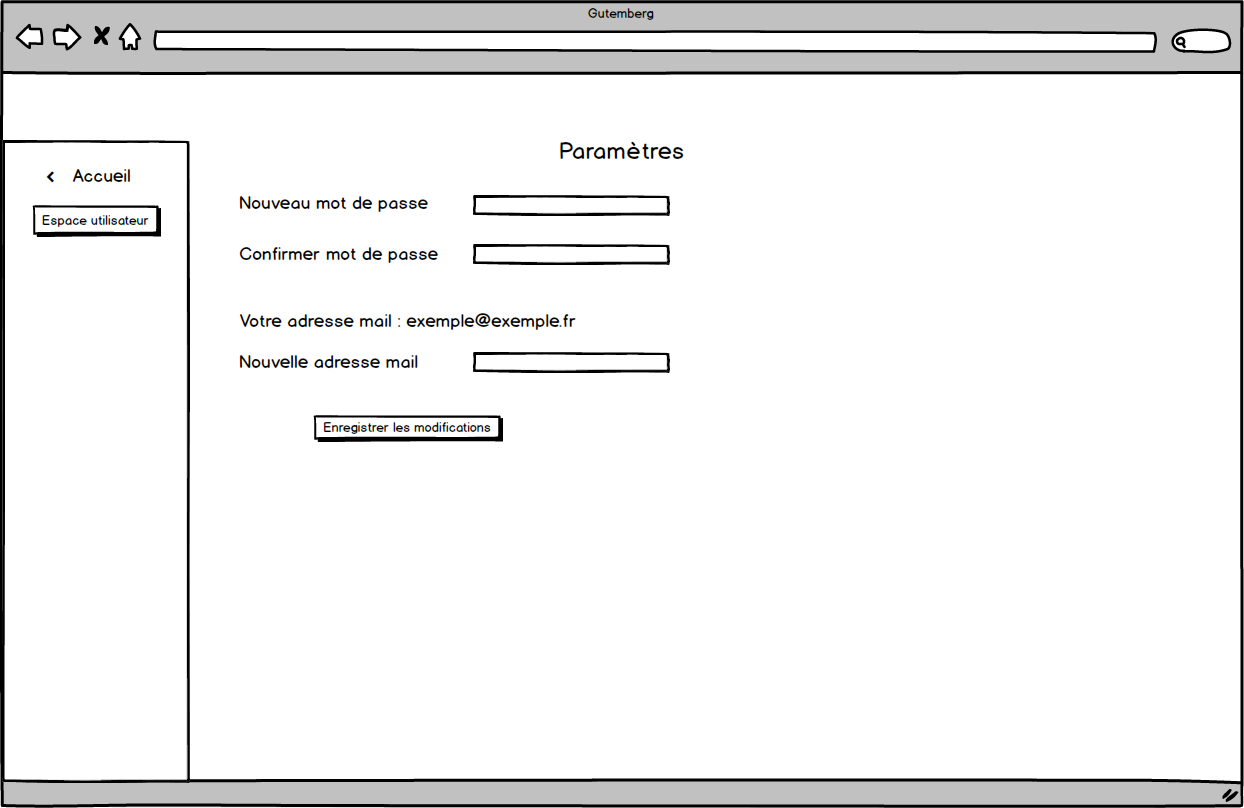
\includegraphics[width=\textwidth]{figures/Parametre.png}
            \caption{Paramètres utilisateur}
            \label{fig:utilisateur_parametre}
    \end{figure}